\documentclass[9pt, oneside]{article}   	% use "amsart" instead of "article" for AMSLaTeX format
\usepackage[left=2cm, right=2cm, top=3cm]{geometry}
\usepackage{cite}
\usepackage[english]{babel}
\usepackage{geometry}                		% See geometry.pdf to learn the layout options. There are lots.
\geometry{letterpaper}                   		% ... or a4paper or a5paper or ... 
\usepackage{graphicx,kantlipsum,setspace}
\usepackage{caption}			% Use pdf, png, jpg, or eps§ with pdflatex; use eps in DVI mode
\captionsetup[table]{font={stretch=1.15}}     %% change 1.2 as you like
\captionsetup[figure]{font={stretch=1.15}} 
\graphicspath{ {images/} }		% TeX will automatically convert eps --> pdf in pdflatex
\PassOptionsToPackage{hyphens}{url}\usepackage{hyperref}
\renewcommand{\UrlFont}{\small\tt}
\usepackage[euler]{textgreek}
\usepackage{verbatim}						
\usepackage{titlesec}
\titlelabel{\thetitle.\quad}
\usepackage{amssymb}
\linespread{1.15}
\usepackage{gensymb}
\usepackage{textcomp}
\usepackage{setspace}
\usepackage[symbol]{footmisc}
\usepackage[version=4]{mhchem}
\usepackage{multicol}
\setlength\columnsep{20pt}
\usepackage{wrapfig}
\setlength{\parindent}{1cm} % Default is 15pt.


% 2 is subsection, 3 is subsubsection
\setcounter{tocdepth}{3}

\begin{document}
\newpage


\begin{center}
\Large{\textbf{Data Provenance Over Computational Graphs}}
\vspace{1 cm}

\normalsize{}
Alan Ransil

Protocol Labs

alan@protocol.ai

\vspace{1 cm}
Updated \today

\vspace{1 cm}
\Large{\textbf{Abstract}}

\end{center}

\noindent Data-driven decision making requires trusted information from many sources to be combined using versioned procedures. Here, we introduce two protocols which when used together allow end-to-end tracing of data provenance and trust over computational pipelines. The first protocol, Transform.Storage, models compute pipelines as symmetric monoidal categories anchored in content-addressed data types. This allows both reproducible and non-reproducible real-world processes to be described as accessible wiring diagrams. Secondly, the Provenance Protocol uses signatures over data to evaluate trust with respect to a community.  While the two protocols may be used independently, together they form a multi-layer system dynamically tracing the flow of trust through complex and multi-party computational processes. We explore how this paradigm can  be applied to real-world use cases.


\begin{multicols}{2}
\setlength{\parskip}{0.1\baselineskip} %Controls vertical space between paragraphs, can re-set line by line
\section{Introduction}

There is a need to establish the end-to-end reasoning behind data driven decisions, and in particular reasoning incorporating data supplied by many parties. Several trends make this need increasingly urgent. First, the trend towards using public and open source data to substantiate decisions increases the utility of expressing these decisions using transparent end-to-end compute pipelines. Second, decisions are increasingly automated with IOT, smart contract and AI subsystems forming parts of the decision making pipeline. Explicitly recording this pipeline is necessary to substantiate trust in the end result. Third, generative AI heightens the need to rigorously track the provenance of data to combat misinformation. Fourth, decisions in critical areas such as environmental sustainability and AI ethics and safety rely on rapidly evolving research which carries an imperative to explicitly lay out methodologies so that they can be reproduced, challenged, improved and rapidly applied. Fifth, the introduction of more powerful and general zero knowledge systems increases the necessity of tracing decisions end-to-end so that proven claims relying on little revealed information can be put into context.

Here we introduce two protocols that together can be used to model end-to-end decisions as modular compute pipelines, reproduce their results if sufficient information is revealed, establish trust relative to norms determined by user communities, and allow subsequent users to reuse or extend these pipelines without sacrificing verifiability. These protocols model compute pipelines in three layers as shown in figure \ref{layeredDataFig1}. The first protocol, Transform.Storage, represents functions as modular, directional relationships between data types. At the Data layer, this defines pipelines as typed datasets on a two-dimensional grid along with functional maps between them. At the Function layer, Transform.Storage represents function definitions coupled with input and output types. The correspondence between these layers is determined by the types of Data on the lower level and the input and output types of Functions at the middle level. The second protocol, the Provenance Protocol, can be used to apply provenance information to data, functions and pipelines and defining bounded trust in each relative to community norms. While the two protocols can be used separately, together they can be used to automatically map the flow of trust evaluated relative to a given Provenance community.

\begin{center}
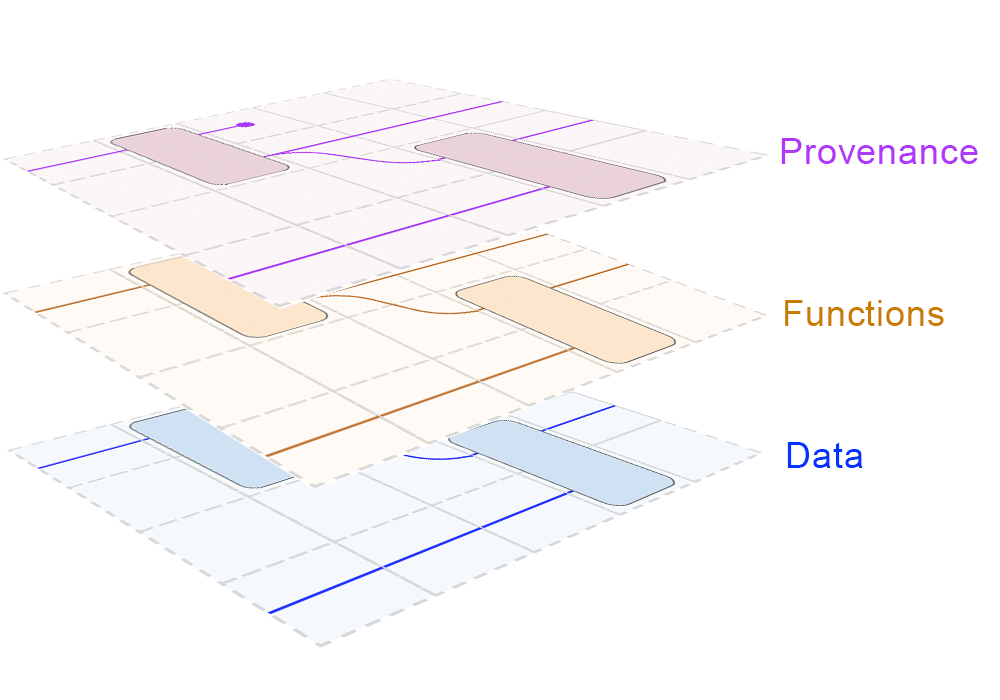
\includegraphics[width=1\columnwidth]{Fig1_20230626}
\begin{flushright}
\captionof{figure}[Three layers of a compute pipeline]{The three layers of a compute pipeline include underlying data, functions operating on the data, and provenance establishing the origins of the lower two layers. Data types establish a correspondence between the data and function layers, while provenance metadata operating over the lower two layers establishes a flow of trust.}
\label{layeredDataFig1}
\end{flushright}
\end{center}

\section{Previous Work}\label{PrevWork}

\subsection{Decentralized Identifiers (DIDs) and Verifiable Credentials (VCs)}\label{did-vc}

DIDs: you do have more control over your key pair

\subsection{IPFS}\label{IPFS}
Tracing decisions end-to-end requires interoperating between work done by many individuals on many different computers and subsystems. The protocols typically used to communicate between machines, such as TCP and https, operate on the basis of location addressing. Under this design pattern, information does not have a persistent identifier and interoperability typically relies on centralized services maintaining endpoints which resolve to network locations. Users of these services typically do not control their own key pairs, which disintermediates them from their data. While the results of these design decisions on market power and centralization of economic control are widely discussed, their implications for data management are similarly profound. Because users are expected to rely on companies to maintain the integrity of their data and market incentives induce vendors to lock in users, it is difficult for developers to write code that traces data across the boundaries between software subsystems.

The Interplanetary File System (IPFS) is a protocol which allows users to address and deliver content based on the cryptographic hash of that content rather than its location on the network. This design pattern, namely using a content address as a URI rather than a location address, is essential for maintaining interoperability and will therefore be used as the basis for data addressing in this work.

\subsection{Symmetric Monoidal Categories}\label{smc}




\end{multicols}
\end{document}  

